\question Two uniformly charged spherical shells are concentric with a point charge at the shared center (see figure). The point charge has a charge $Q_{pt} = -4\ \mu$C. The inner shell has a total charge $Q_{inner}=2\ \mu$C, and radius $R_1=0.2$ m, and the outer shell has a total charge $Q_{outer}=-2\ \mu$C and a radius $R_2=0.3$ m. The shells are separated by vacuum (they are not in conductive contact).

\begin{figure}[ht!]
	\centering
	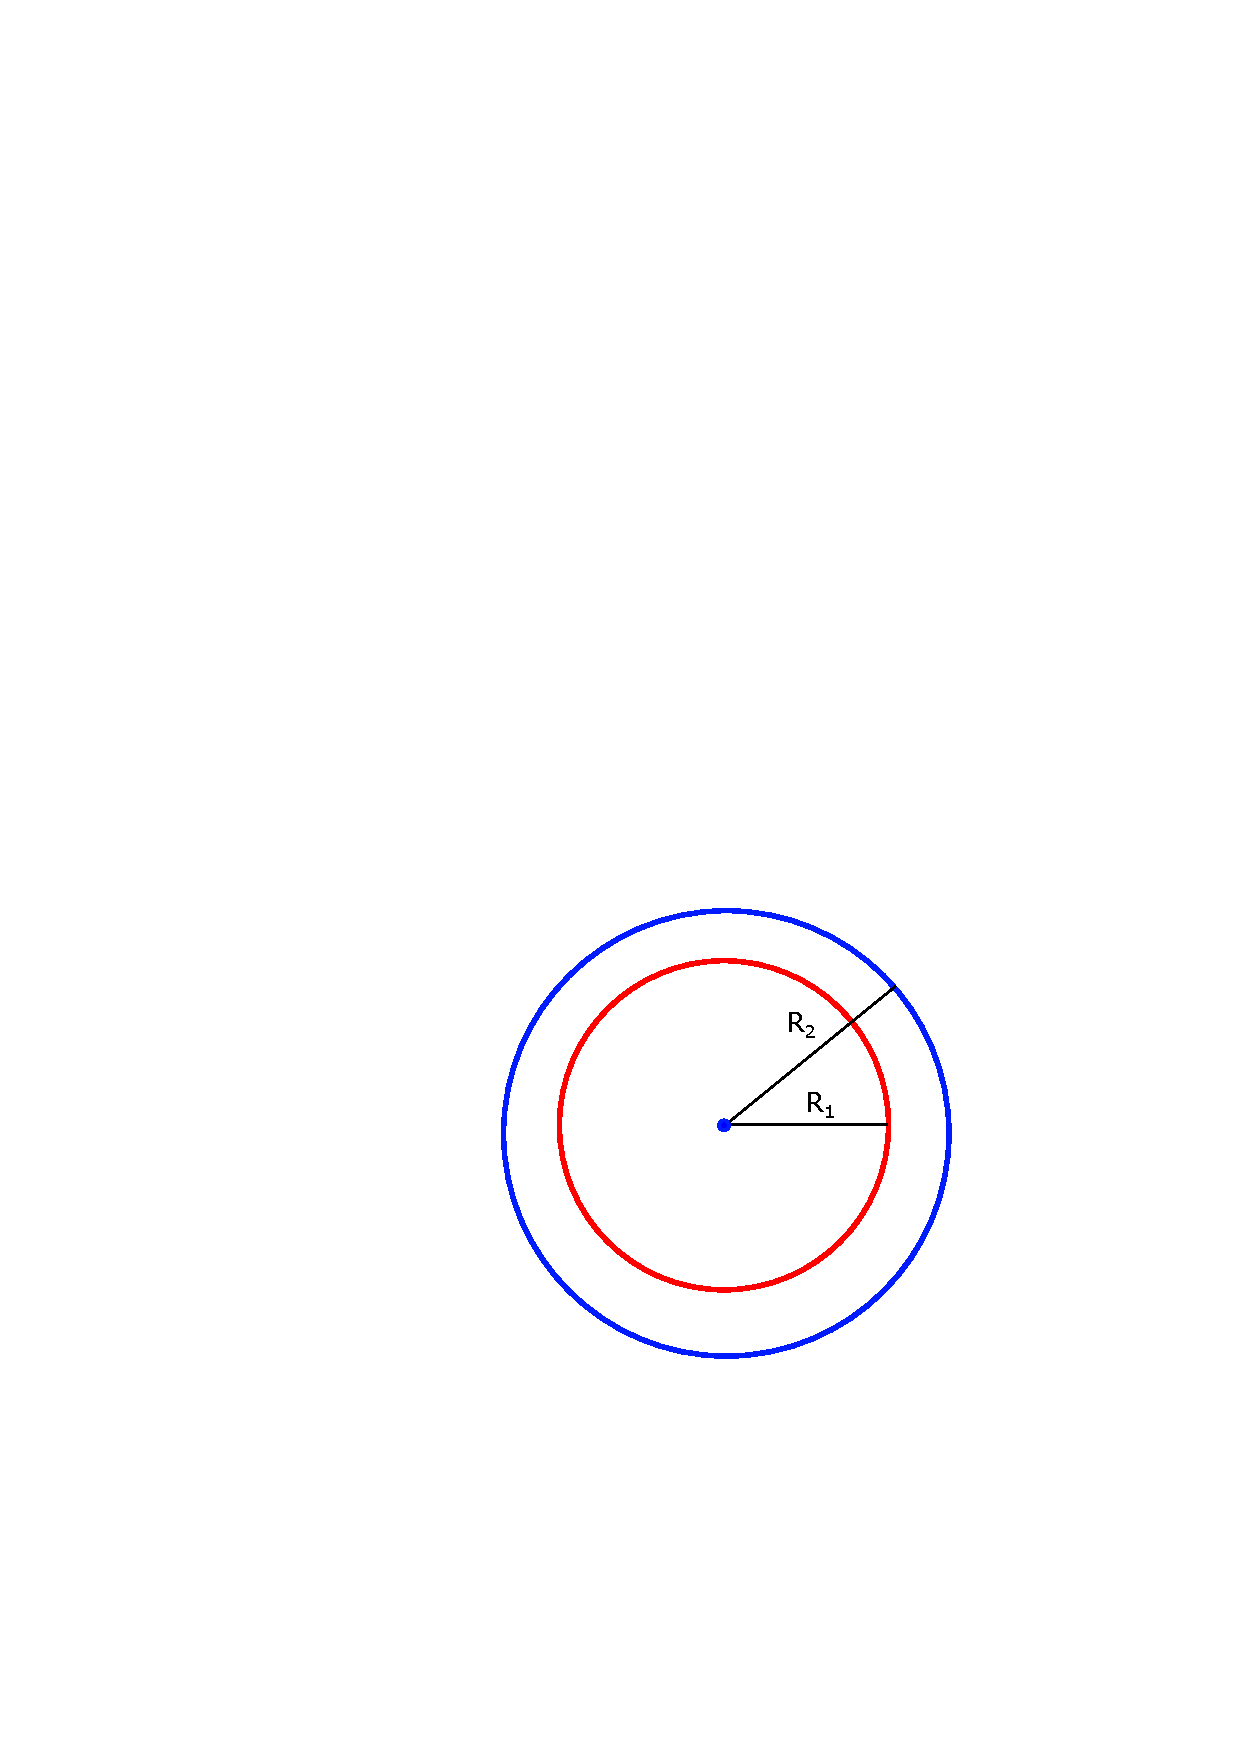
\includegraphics[width=5cm]{concentric}
\end{figure}

\begin{parts}
\part What is the potential difference between the surfaces of the inner and outer shell?
\part What is the magnitude of the net force experienced by a proton placed 0.5 m away from the center of the shells?
\end{parts}